
\chapter{Use case UZGent}
\label{sec:use_case_uzgent}
To put the theory of speculative decoding into practice, this thesis looks at a use case for RAG at the UZgent. This chapter starts with a description of the use case. Then the technical implementation is uncovered, detailing how the architecture of the RAG system works.

\section{Description of use case}

\begin{figure}[h]
	\centering
	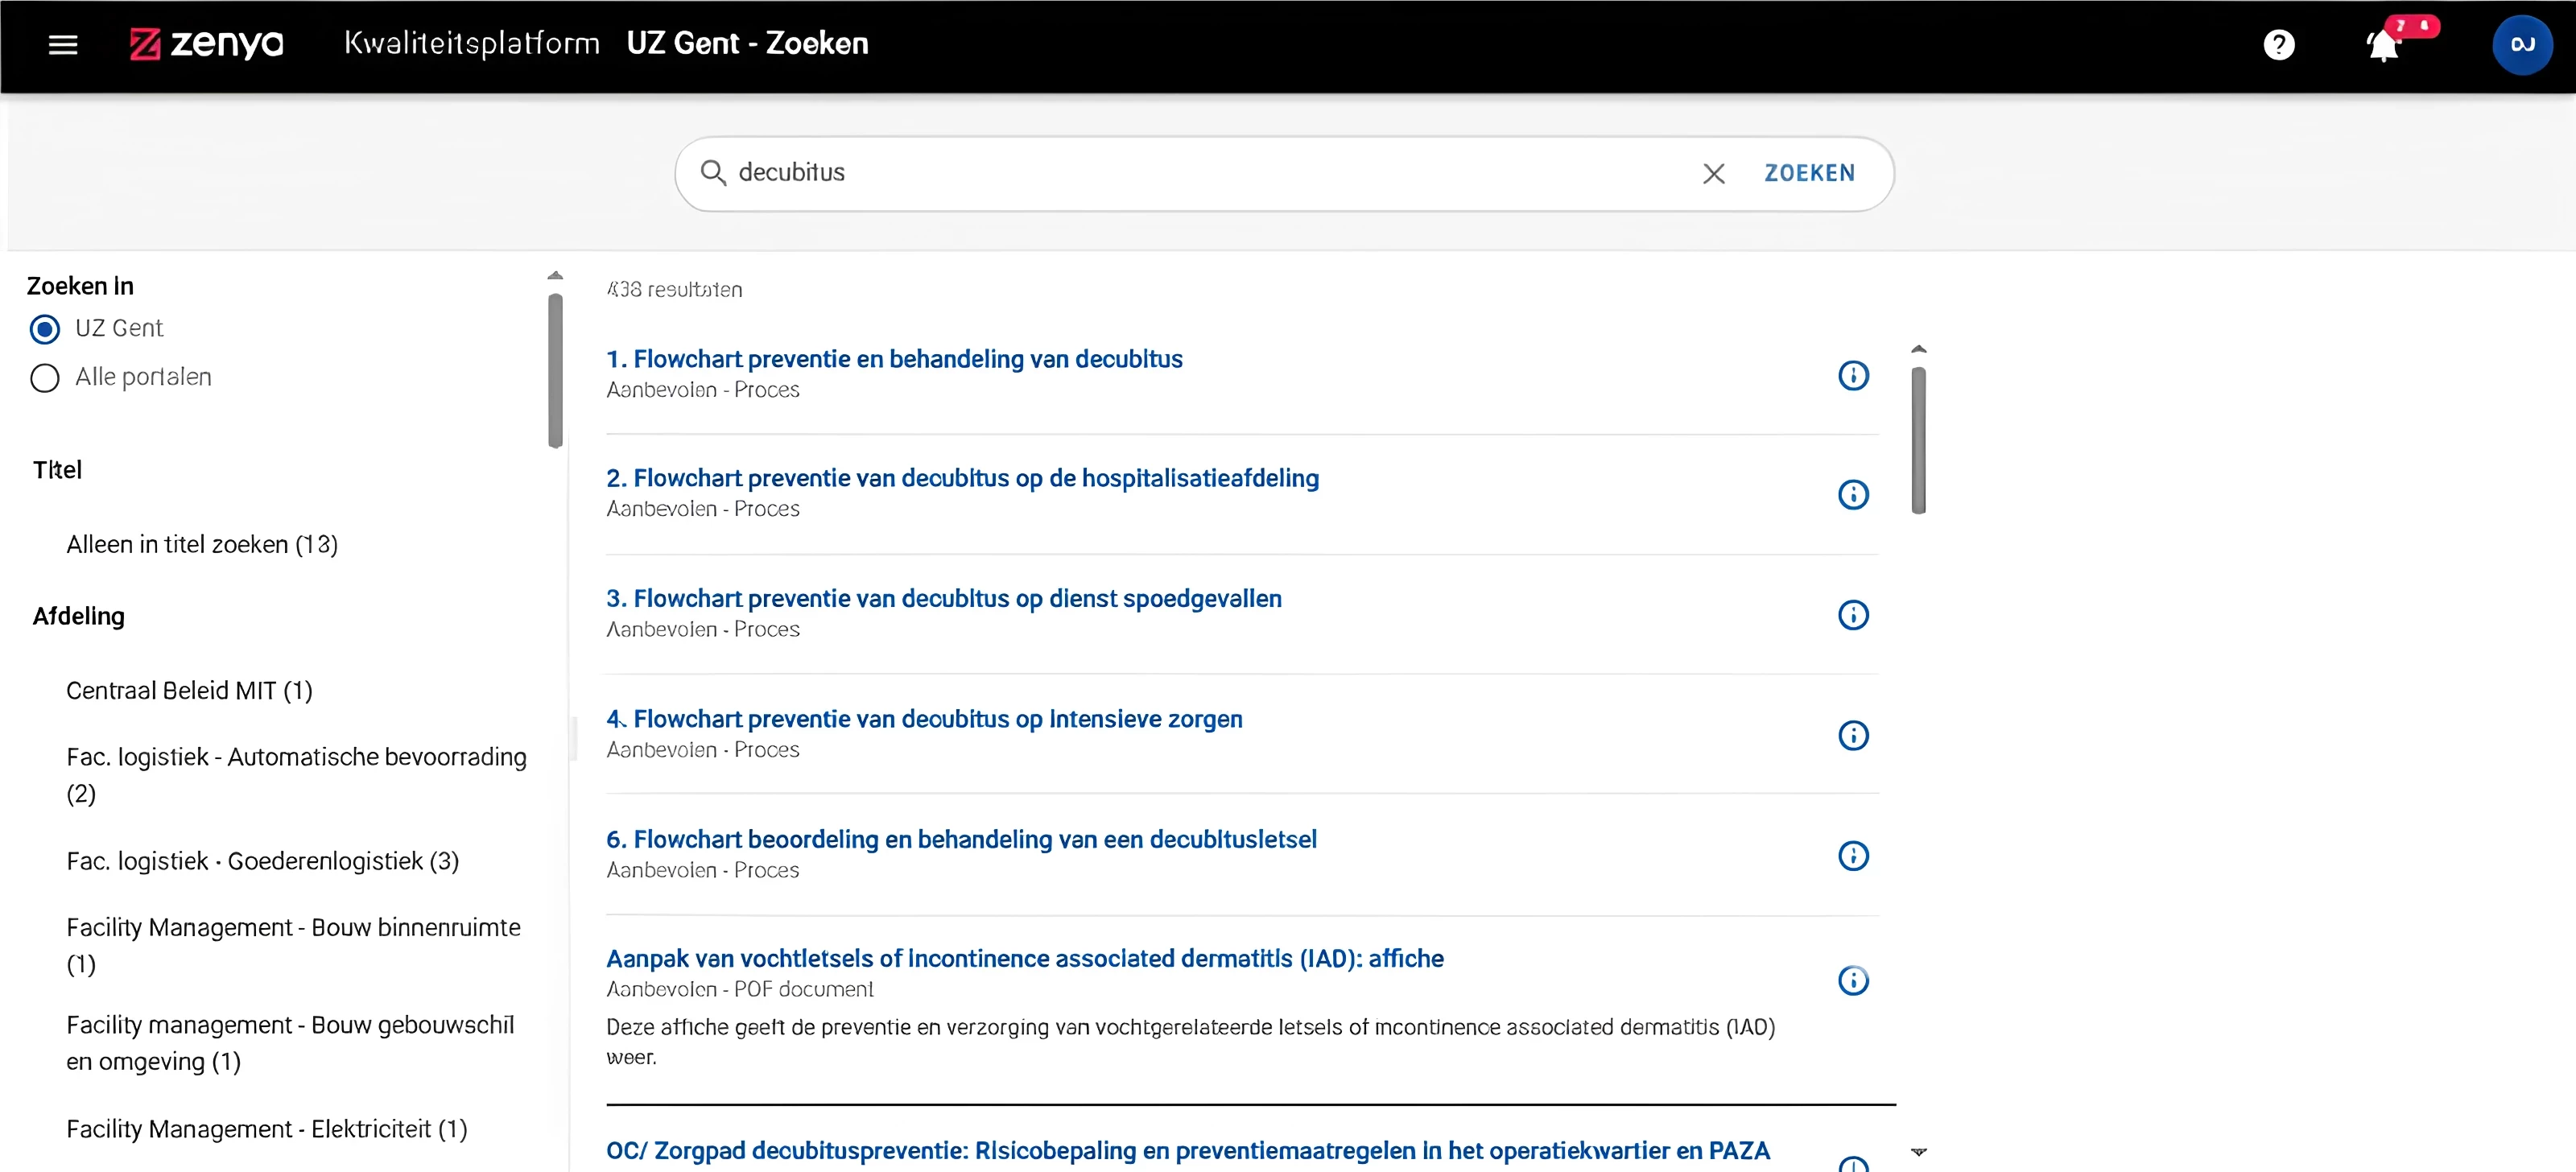
\includegraphics[width=\linewidth]{fig/zenya.png}
	\caption{Screenshot of Zenya, the current system doctors use to search procedure documents.}
	\label{fig:zenya}
\end{figure}

In the UZGent, there is a system, Zenya and it contains many documents often needed by healthcare professionals. To work with the tool, one must either be guided or have enough experience themselves in order to get the document they need to read. Also, the documents can be quite lengthy, while often only a very specific part or summary is necessary. This makes the perfect use case for a RAG system. In this RAG system, the user first poses a question. Then the retrieval fetches the relevant documents based on a deeper understanding than the current keyword-only search. Finally, the relevant part of the document is read by the LLM and used to answer the question in a concise way. This description was rather general about RAG, however each use case is different and has different requirements. To get a grasp of the details of this use case, many involved people were interviewed. A summary is given below.

The answer to each question is in one single document. This already simplifies the RAG complexity. It also means that the retriever has only one document to find as the ground truth. However, this can still be multiple chunks long, sometimes requiring a summary of large parts of the document.
The question will be in natural language, rather than keywords as it used to be with Zenya. However, the language can contain abbreviations, short rather incomplete sentences. This is because the healthcare professional often needs the answer quickly.
The system should know when it does not know. It is very important that when there is no answer in the database, it is able to detect this and answer accordingly.

\section{Technical implementation}
In this section, we list the technical details of our implementation. Following chronological order, the documents need to be preprocessed first. Then, the retriever must find the right chunks and the generator will produce an answer. Finally, some postprocessing will make the result more accessible to the end user. As a guide through this section, Figure \ref{fig:dataflow_graph} shows the high level data flow graph that makes RAG possible.

\begin{figure}[H]
    \centerline{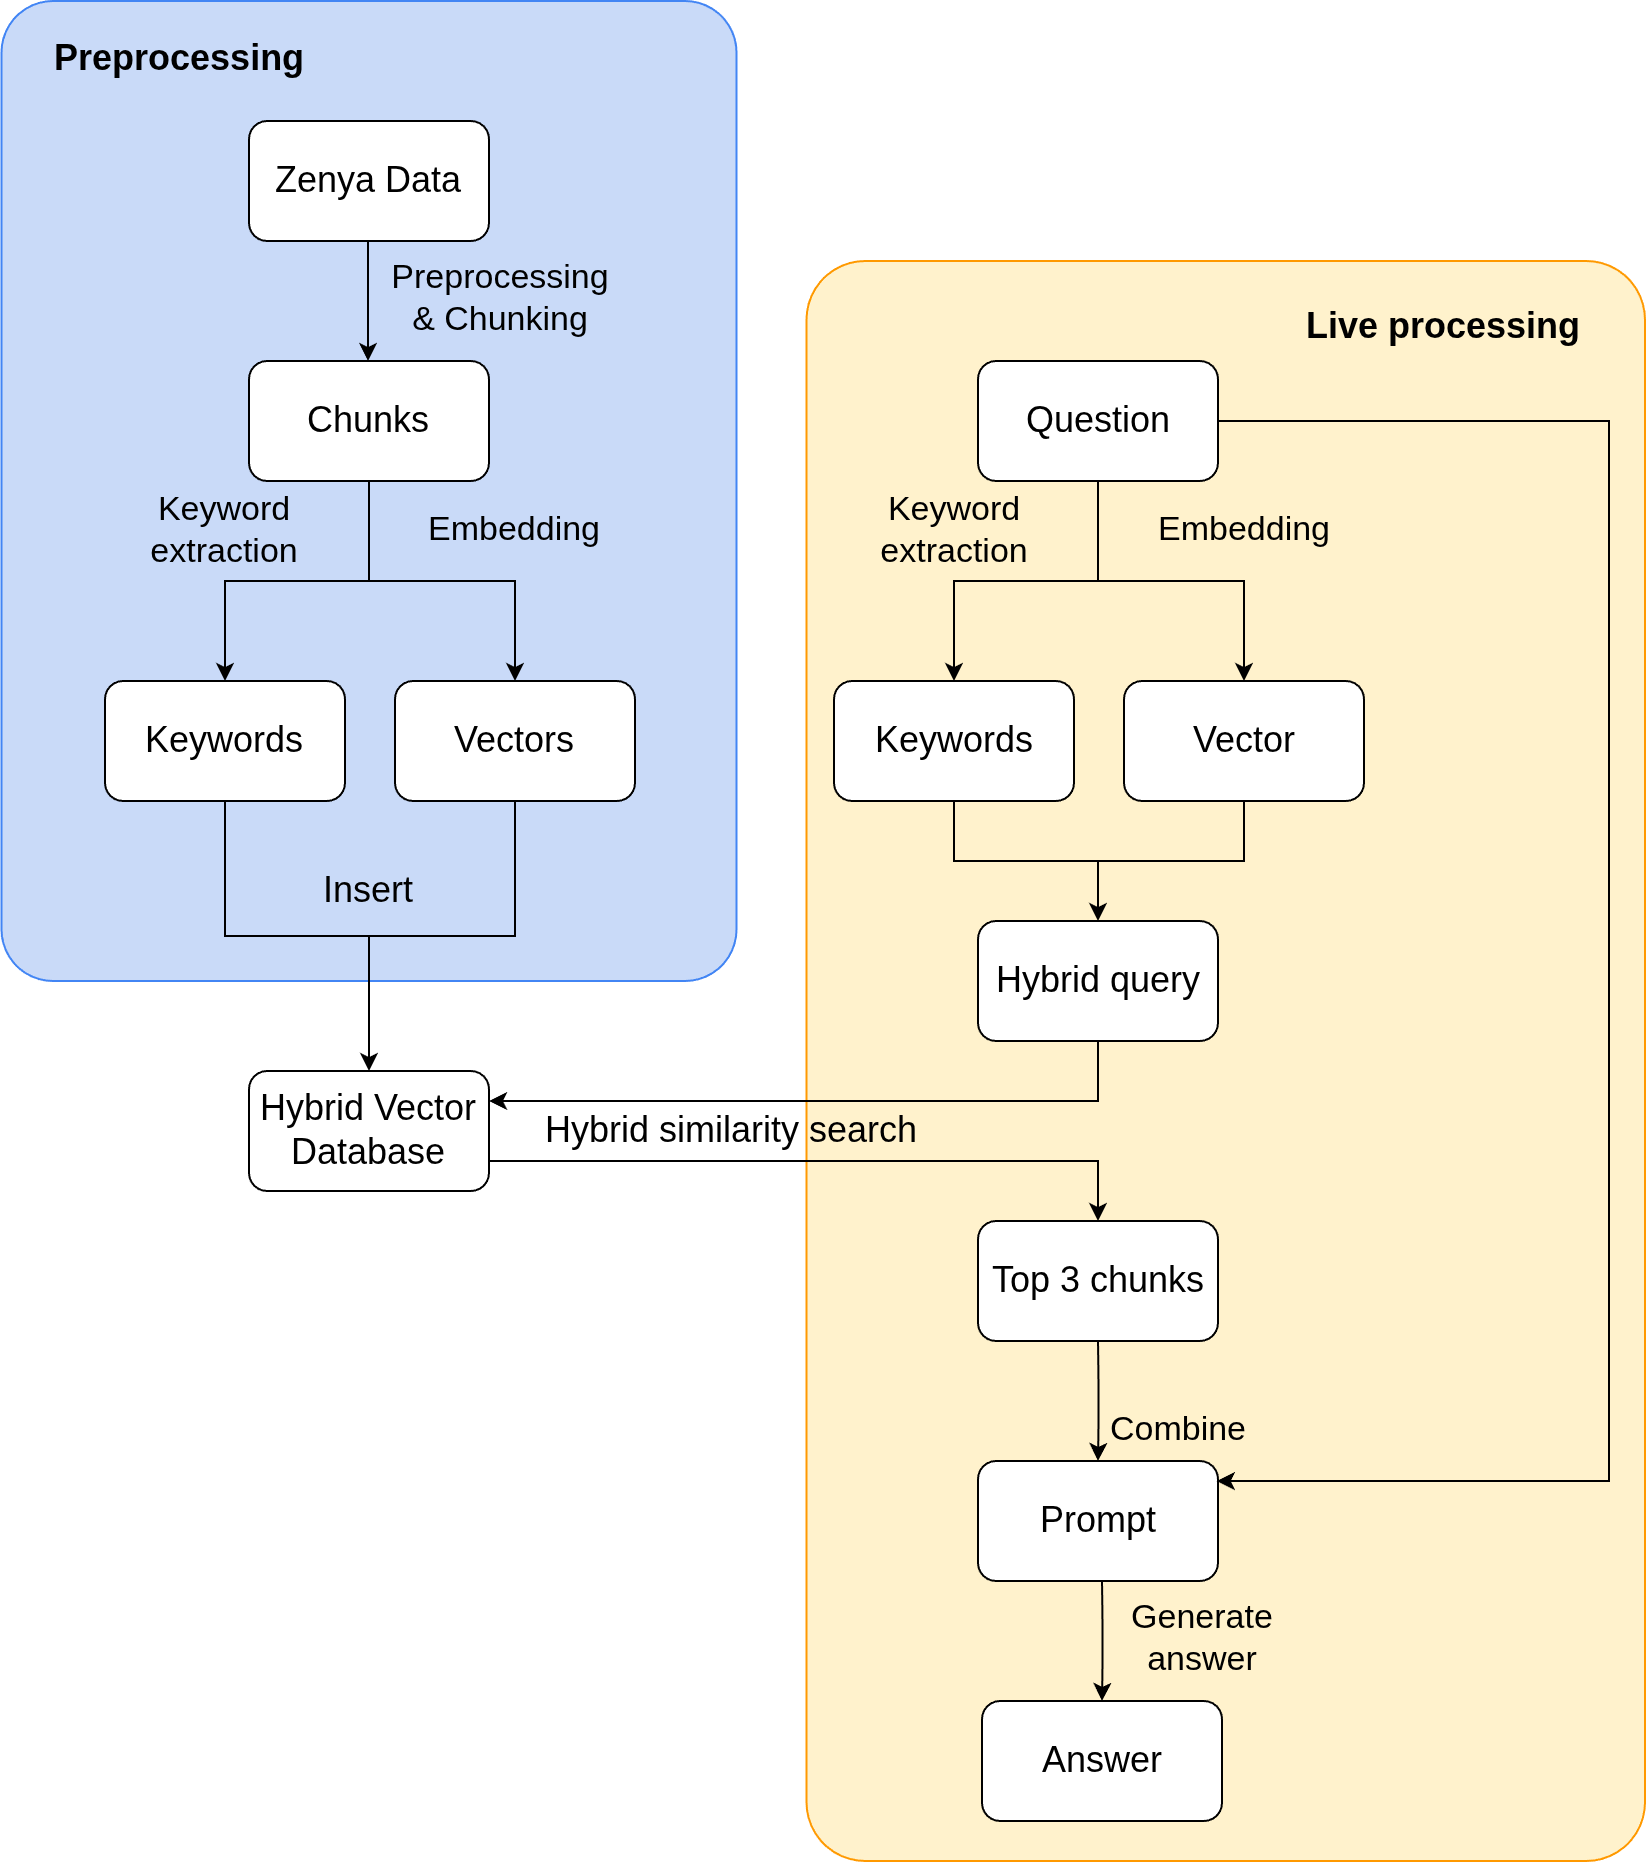
\includegraphics[width=0.8\linewidth]{fig/dataflow_graph.png}}
    \caption{The data flow graph, which shows how the data and input question lead to a final answer. The graph is visually split to indicate the difference in time. The blue part fills the database and as this data is constant, it can be calculated in before. So practically, this preprocessing is done before the system goes live. The orange part shows the live processing that is repeated for each new question that comes in.}
    \label{fig:dataflow_graph}
\end{figure}

\subsection{Preprocessing}
To start the preprocessing, one must first know what format the data will have. The database of Zenya contained many file formats: pdf, docx, excel, ... This heterogenity is not desirable for building a quick proof of concept (POC) in the scope of this thesis. Yet, it seemed that the majority of the files were pdfs and docx, most of which contained primarily text. This is visualized in Figure \ref{fig:file_type_distribution}. The first conclusion is that pdfs and docx are important, while the rest can be ignored in a simple POC. Also, the data exporter made it possible to convert docx to pdf and for simplicity, this was used, such that the input data was as homogeneous as possible. The python module PyPDFDirectoryLoader of the langchain\_community package  provides very concise code to parse these pdfs and provide the text in them. This text is not directly used, because pdfs (like most other formats) contain much textual noise. One example is the character "$\backslash$" which often appears in places one cannot find visually inspecting the pdf. For this reason, a pdf text cleaner scans all text and strips the text down to the real content. After this cleaning, mostly natural language remains in the text. To clarify, an example is given in Figure \ref{fig:pdf_clutter}

\begin{figure}[H]
    \centerline{
\includegraphics[width=0.5\linewidth]{fig/pdf_clutter.png}}
    \caption{Example of a non-informative pdf page in Zenya. Despite being almost empty, the pdf parser extract over 2500 hidden characters.}
    \label{fig:pdf_clutter}
\end{figure}

\begin{figure}[H]
    \captionsetup{justification=centering}
    \centerline{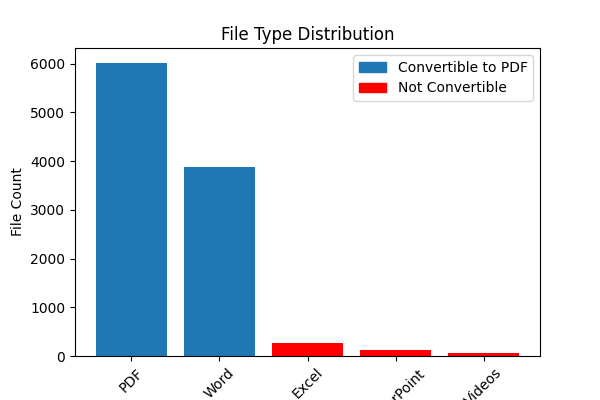
\includegraphics[width=0.7\linewidth]{fig/file_type_distribution.png}}
    \caption{The file type distribution of Zenya documents.}
    \label{fig:file_type_distribution}
\end{figure}

With the actual text available, the next steps are those typical to RAG. 

\subsection{Chunking}
First, the text of each pdf is split into smaller pieces, chunks. This chunking helps in multiple ways. Good chunking can make the pieces of text more bite-sized, such that the embedding model can interpret it better. Also, RAG does not always need to read the full document, but rather the relevant part, so chunking also limits the amount of noise around the retrieved information. There are some choices necessary to do chunking successfully. The optimal chunk size, the first choice, depends on both the dataset and the embedder. It is usually helpful to match the chunk size with how long one thought is in the dataset. Next to that, an embedder is trained on a certain input size and they work better when working in similar sizes of new input. Empirically, it was found that approximately 800 characters is optimal for the use case. 

The next option, is to use overlap. When splitting text it is impossible not to break an ongoing thought at any point. To make sure this cut in the text does not lose the information in that passage, overlap is often used to make sure this context helps both the previous and following chunk. The exact number did not seem to matter enough to make significant changes to the validate score, so we chose a 20\% or 160 characters overlap.

\begin{figure}[h]
    \captionsetup{justification=centering}
    \centerline{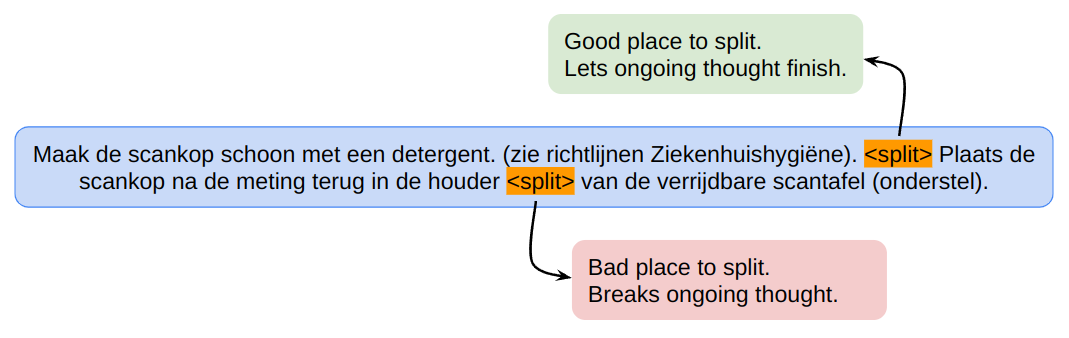
\includegraphics[width=1\linewidth]{fig/good_split_bad_split.png}}
    \caption{The difference between a good and bad point to split, applied on content from Zenya.}
    \label{fig:good_split_bad_split}
\end{figure}

With this target chunk size and overlap, one still needs to decide where to cut the text. While deterministically stepping by 800 characters at a time would be a simple method, it can cut through thoughts, or even worse: words. Figure \ref{fig:good_split_bad_split} shows the difference between a good and a bad split. To solve this, the RecursiveCharacterTextSplitter of langchain\_text\_splitters splits the text recursively. Each time, it tries to find the most splittable characters until the desired chunk size is approximately met. Practically, this means that a hierarchy is followed where, for example, the new line character "$\backslash$n" is prefered over a space " " to split on. With this last choice made, the chunks can be extracted.

\subsection{Retrieval}
With the text split into chunks, the next step is to retrieve the right chunks for a query. This is the hardest part for a reasonable proof of concept. A clear distinction is made between what worked and what did not.

\subsubsection{Effective retrieval techniques}
In this part, the retrieval techniques are listed that are actually used in the final RAG system. In other words, the methods below all successfully made the retriever return better documents.

As explained in Chapter \ref{sec:rag}, retrieval is always based on a similarity search. In this case, the similarity search is a hybrid search, meaning classical methods (BM25) and dense retrieval (embeddings) are combined. This hybrid search was supported by the python package weaviate, with accompanying vector database (see Figure \ref{fig:architecture_docker}). To combine the scores of two methods, the separate scores are first scaled such that the minimum is 0 and maximum is 1. Then they are combined with a weight: $\alpha \cdot \text{dense score} + (1-\alpha) \cdot \text{BM25 score}$. $\alpha$ has a default value of 0.7, focussing most on the embedder. By coincidence, this was found to be the optimum for the use case too. For BM25, some parameters are available to tune, but typically the defaults suffice. In this case the defaults were also used as implemented by weaviate.

The largest effort went into dense retriever. Not only are there typical parameters to tune, but since the rise of LLMs a whole new realm of tricks have allowed retrieval systems to push it to the limits. The discussion starts with the classical choices.

To start, we first need to find a good embedding model. A pragmatic approach is the only way not to get lost in the thousands of embedders, available on HuggingFace. To compare these embedders, a good benchmark is necessary that represents the Dutch, medical use case somewhat. Beyond MTEB, no reputable benchmarks were found to give a fair and insightful comparison between embedders. And needless to say, MTEB differs much from the intended use case. Surprisingly, Reddit turned out to be the most useful source of evaluations of models \cite{reddit2025embedding}. This is likely, because Dutch is a niche language and a more professional comparison is not worthwhile. In that reddit discussion, they mention the embedder that performs best on our tests. The model is called BGE-M3 and it is a multilingual embedder. This property has proven to be the most important among all tested embedders. While a specialized model exists specifically for multilingual medical data, BioLORD-2023-M \cite{remy2024biolord}, we hypothesize that the BGE-M3 model performs better based on sheer size. BGE-M3 is 568M parameters large, while BioLORD-2023-M has only 109M parameters. Other factors could be at play too, but no deep analysis was done: whatever works works.

With this setup, we ran the first tests to analyze the performance and the weak spots of the current model. A recurring error was that the embedder did not match on chunks that were in the middle of a large explanation. A typical example would be a document where the title contains the important keywords such as "hemathology" or "oncology". As these documents were made for human readers, the rest of the full pdf assumes that the reader remembers that context. An example of a chunk with too little context inside is shown in Figure \ref{fig:out_of_context_zenya_doc}. So the chunks in se do not contain enough information to properly match with the query. As a rather quick solution, we appended the title to each chunk before being embedded. The structure is as follows: \verb|f'Titel: {title}\nTekst: {cleaned_text}|'. This simple method yielded approximately a 0.08 gain in MRR (explained in the following paragraph), which is an enormous boost.

\begin{figure}[h]
    \centerline{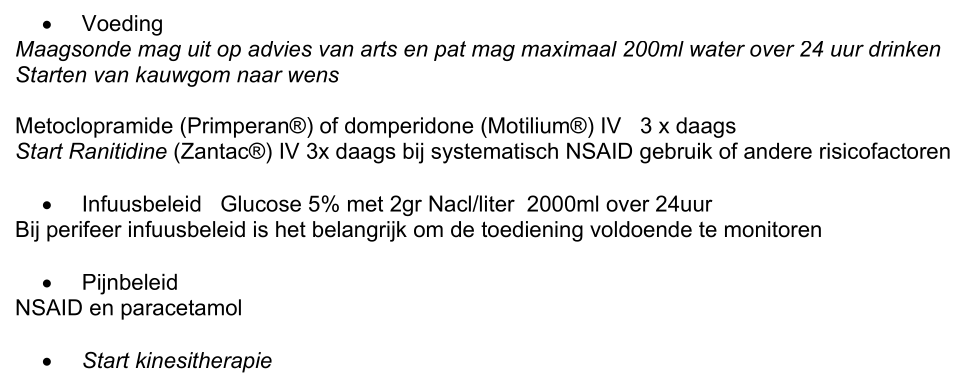
\includegraphics[width=1\linewidth]{fig/out_of_context_zenya_doc.png}}
    \caption{Chunk of a pdf with the title ``Zorgpad invasieve blaastumor robotgeassisteerde cystectomie met neo-blaas''. The chunk does not contain enough information to place it into context. The title clearly adds some necessary context.}
    \label{fig:out_of_context_zenya_doc}
\end{figure}

To objectively compare different models, it is important to choose the right metric for the job. In this thesis, the goal of the retriever is to get one piece of information and to make sure that piece is ranked as high as possible. The logical metrics to use in this case are Hit@k and Mean Reciprocal Rank (MRR). Hit@k is the probability that a relevant document is in the top k results. So Hit@3$=0.7$ means that a relevant document is in the top 3 retrieved documents for 70\% of the times. The MRR is defined as $\frac{1}{U} \sum_{u=1}^U \frac{1}{rank_i}$, with the rank defined as the place of first document that is relevant, as shown in Figure \ref{fig:rag_rank}. In the best case scenario, a relevant document is retrieved on place 1, resulting in rank 1. As the MRR is the mean of many such ranks, the best possible MRR is 1. Thus, the MRR ranges between 0 and 1.

\begin{figure}[h]
	\centering
	\captionsetup{justification=centering}
	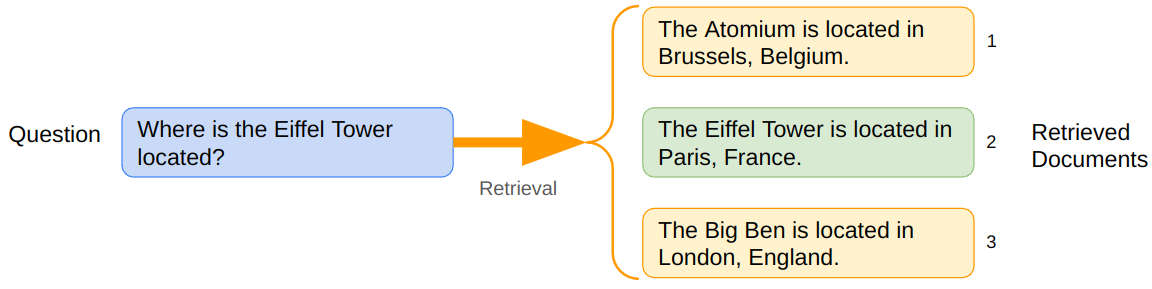
\includegraphics[width=0.9\linewidth]{fig/RAG_rank.png}
	\caption{Example of a retrieval to explain the rank. For this question, there is clearly one relevant document retrieved: the second one. This makes the rank of this retrieval 2.}
	\label{fig:rag_rank}
\end{figure}

We then repeated the analysis to find the common causes of errors again. The most common source of mistakes was medical synonyms and abbreviations. This is not too surprising as the model was not trained for this. In fact, it is somewhat of a miracle that the model works this well without actually having a clue what most questions are about. Practically, this means that questions with uncommon terms, medical abbreviations or even abbreviations specific to the UZGent often did not match well with the intended chunks. This issue is quite fundamental and to the best of my knowledge, the only real solution is to fine-tune the embedder. This was out of scope for this thesis, so it is listed as future work.

\subsubsection{Ineffective retrieval techniques}
Of course, many methods were tried that did not lead to improvements. These methods are listed below. It is important to note that these methods do work in other settings and that it is specifically for this use case that the methods did not work. So either the method was not fit for this specific dataset, or it required larger models than what could be run locally on the UZGent servers. In other words, this chapter indicates what a future developer should not try again for this specific use case if the setup does not change.

One such method that did not work is to \textbf{search chunks hierarchically}. To see whether this was a technique worth considering, the implementation started with a very simple approach. First, the retriever fetches the chunks as usual, but then the scores are aggregated per document. Afterwards, the idea is to find the right document first before taking the best chunks out of that document. To see whether this method was worth considering, we considered the document-MRR as an indicator. The document-MRR was lower with aggregation than without it, which means it made the retrieval worse. So this idea was dropped. However, the principle of hierarchical search is still promising for future work, when more time and data is available. UZGent has metadata for each document (that was not available during the thesis), which could strengthen this method. For example, during practical usage multiple doctors and nurses gave the feedback that the retrieved chunks were very reasonable and contained the right information, but for another function. E.g. paediatrician got very relevant results, but for adults rather than kids. To help guide the model, the function of the user could be given to the retriever and the metadata could say for who which document is intended. This way either documents can be filtered or given extra score for being fit for the specific user asking the question. In conclusion, gathering this data and implementing hierarchical search is also future work.

The \textbf{small-to-large method} also did not yield any improvements. The idea behind small-to-large is that the matched chunk is similar to the question, but not necessarily the answer. So certainly for small chunk sizes, the answer is to be expected before or after the chunk. And thus the solution is to retrieve a small chunk and then just expand, gathering also a piece before and after the retrieved chunk. During the process, this was first relevant, because the first tested models required small chunk sizes. Then, the final embedder we used was optimal for large chunk sizes, so this technique became less relevant. However, it later seemed that even for the large chunk sizes, the answer was often hidden before or after the chunk. This time, though, the chunks started crossing page boundaries and the used pdf parser made it harder to cross that border. While this is not the largest effort to fix, it was still not implemented. The most important reason was that the expected gains were for the generator rather than the retriever and at the time it already became clear that there is probably no future for the generator (as discussed in Section \ref{Ethical considerations}).

Another method that failed in this particular use case was \textbf{reranking}. The reranking method starts as usual: the query is embedded and a similarity search finds the top-k most relevant chunks. Then the reranker model compares the query to each single chunk to give a relevance score. So the original order is dropped and replaced by the order that the reranker finds most relevant. The reason that this should work better, is that classical retrieval has an intermediary step of an embedding which implicitly encodes similarity. Learning the similarity directly should be an easier task and thus these models should perform better. The reranker BGE-Reranker-v2-M3 \cite{chen2024bge} was tested, as the embedding model of the same publisher performed so well, but the MRR went down when reranking. Further analysis was beyond the scope of this thesis and thus the idea of reranking was also left out.

While \textbf{rechunking} seemed promising too, it did not deliver improved scores. Rechunking works as follows: first the classical retrieval is performed and then the retrieved chunk(s) are split again in even narrower parts. These new parts are again scored based on their similarity with the query to find the best match with a much smaller granularity. This works well in cases where the goal is to find one small piece of text. However, this seemed to conflict with the goals of the application. Consider the following dummy question that is based on a real Dutch question the doctors asked: "How much Vancomycin do I give to a 46-years old patient with a viral infection?" The answer could be as simple and short as "15 mg/kg", but if we single out that specific piece in the retriever, we might miss crucial information that the LLM would not miss. One problem could be that this answer came from the document "Vancomycin for patients younger than 18". Even common metrics such as RAGAs' \cite{es2024ragas} faithfulness would praise this answer as it was grounded in the retrieved chunks (though it was the wrong chunk and wrong document). To further dive into the possible problems, the question was a trick question. Vancomycin is for bacterial infections rather than viral infections \cite{vancomycin_wikipedia}. Even though this is a dummy example, we found that in real cases the critical context was often found far above of below the retrieved chunk. So the perfect answer of ``Do not use Vancomycin for viral infections.'' has very low chances of actually being the output of the chatbot with short contexts. To solve the problem of missing context, one could just try to give the whole document to the generator. This is not the solution, because the missing context is often times implicit as the writer of the document thought of it as common sense, which the generator does not have. Specifically in this case, the limitations of a 9B model also became clear when too much context was given.

\textbf{HyDE} \cite{gao2023precisehyde}, \textbf{Step-Back Prompting} \cite{zheng2023takeastepback} and \textbf{splitting the question} (methods discussed in Section \ref{sec:pre_retrieval}) all could not live up to the expectations. While these are proven methods in general use cases, this particular case was somewhat different. We analysed why these methods failed and found out that the added value was much smaller than the noise the LLM added. Often times the LLM did a good job at making extra queries for the retriever, but sometimes it was confused by either a lack of general understanding or a lack of medical knowledge. In the end, the average retrieval score went down, proving that the added noise was too large.

\subsection{Generation}
After the retriever has found a list of possibly relevant chunks, the generator uses that information to generate an answer. To optimize a generator, there are broadly speaking two common options: making the prompt better and making the model better. The latter option is usually work-intensive and resource-intensive, making it out of scope for this thesis. By consequence, the following paragraphs will discuss only prompt engineering techniques used in the application.

The first technique is to properly separate pieces of information. The pragmatic approach was to use the first separation technique that the generator seemed to handle well. This turned out to be the following style:
\begin{verbatim}
[begin context]
Jij bent een dokter. Jij kent alle medische procedures van het UZGent.
[einde context]
[begin documenten]
{context}
[einde documenten]
[begin vraag]
{query}
[einde vraag]
[begin antwoord]
\end{verbatim}
This is of course the prompt for the G in RAG. As stated before, the generator was also used in other settings, but the same style with brackets was kept. As a sidenote, the context of ``You know all medical procedures of the UZGent'' might seem weird, motivating the generator to answer possibly more often than it should. However, without this part the model seemed to be fine-tuned to say it cannot answer medical questions. So it is a little hack to get an answer at all.

The second technique is few-shot prompting \cite{brown2020languagepromptengineering}. This uses in-context learning to show the model what typical input is and the corresponding model answer. At the time of development, the prefered answer of the full pipeline was still unclear, so few-shot prompting was not used. But for other techniques, such as HyDE, it did yield improved results (though still not good enough). 

\subsection{Postprocessing}
The last part of the pipeline is to make the output presentable for the end user. Figure \ref{fig:chatbot_zenya} shows the user interface with an example question and answer. Not only do we present the answer, but also the used context and where it came from. To this end, the plain text is searched again in the original document (pdf) and highlighted. And as a nice addition, the pdf is automatically scrolled to the highlighted part. 

\begin{figure}[h]
    \centerline{
\includegraphics[width=0.7\linewidth]{fig/chatbot_zenya.png}}
    \caption{Screenshot of the user interface of our chatbot.}
    \label{fig:chatbot_zenya}
\end{figure}

\section{Application diagrams}
The department of ICT at UZGent was very enthusiastic about this project and they showed interest to understand how the web application was made. We made the following diagram to clarify what was going on in the background. Figure \ref{fig:architecture_docker} explains the whole application in high level components. While a simple diagram now, this used to be different. We put significant effort into containerizing each component, making them as independent as possible and building those efficiently to reduce build time. The orchestrator is simply a github repository that contains a docker compose file and some necessary configurations. This docker compose will then spin up the docker containers. Most of them are straight from an image, but some of them are built with local code. The RAG container is built from local python code and it runs the API. The API's input is a question and it returns the answer with corresponding chunks. The website is also built from local code and it is a typical chat interface that forwards questions to the API. The reverse proxy uses the well known nginx in docker to allow https connections to the website. The vector database is also a default weaviate container, just like the database is a default postgres container. Finally, vLLM also supports a containerized version making it very easy to host LLMs in a scalable way.

\begin{figure}[H]
    \captionsetup{justification=centering}
    \centerline{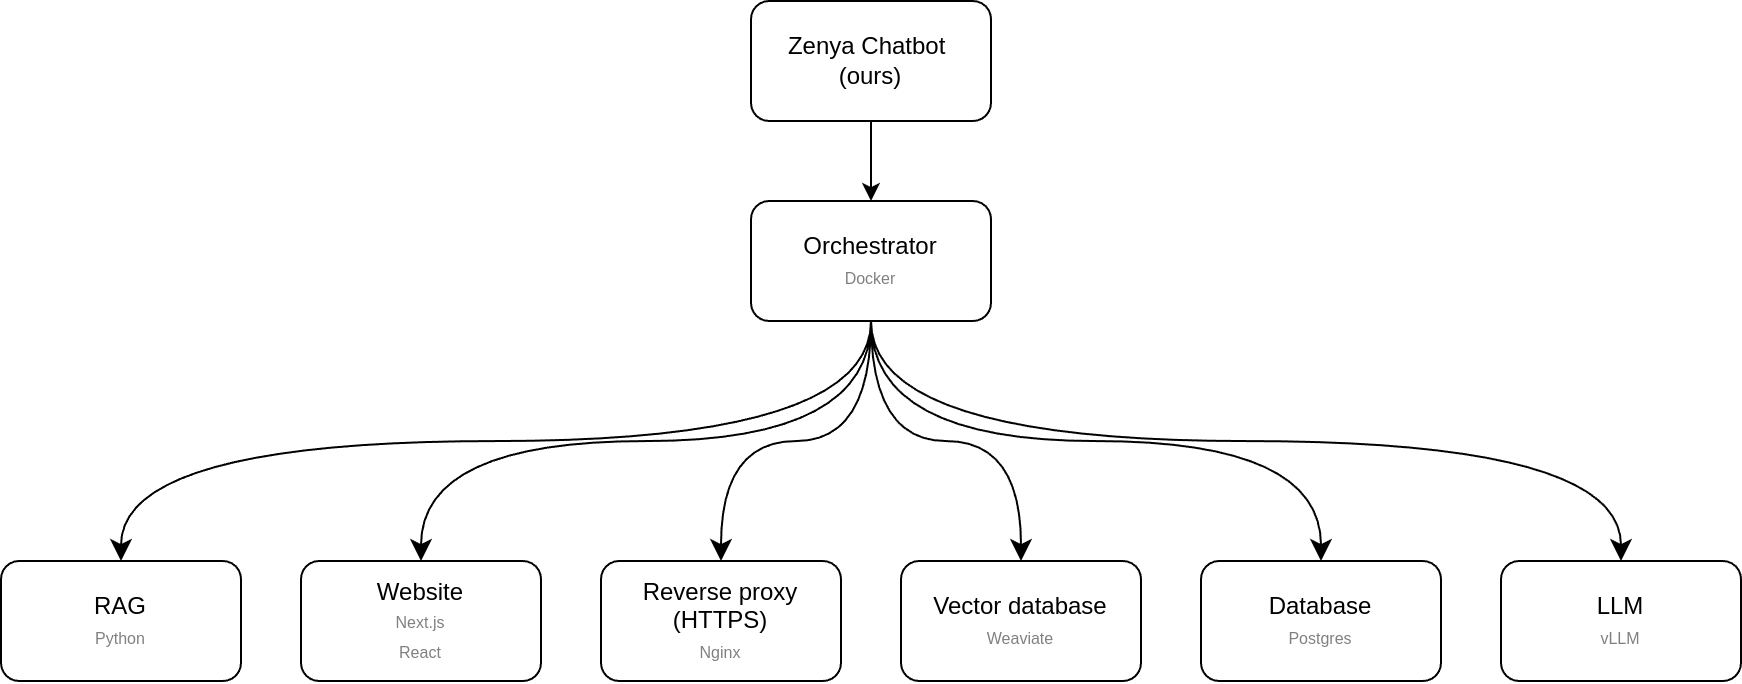
\includegraphics[width=1\linewidth]{fig/Architecture Docker.png}}
    \caption{A high level diagram that lists the different docker containers of our application.}
    \label{fig:architecture_docker}
\end{figure}

\section{Test results and feedback}
This section discusses both the test results and the informal feedback gathered during the sessions.

Before going into the test results, some caveats must be pointed out. First of all, this test data is important for future use at the UZGent, as they want to use it to evaluate all possible competitors that claim they can do better than the current system, Zenya. This means a validate set is necessary to hand over to the competitor and a test set to keep for themselves. As the writer of this thesis is both the person gathering the data, making the split and also testing his system, this is something of a violation against best practices. Thus, the UZGent will have to trust us not to make any decisions based on the test set.

The next problem, is that the test set turned out to be quite unclean. For example 20\% of the ground truth documents were derived from the context. While this would work if every tester followed the instructions perfectly, testers remain human and make mistakes. Thus sometimes this derived ground truth is not actually right. Additionally, 8\% of the questions were left without any clue what the ground truth would be. Ideally, these questions should be revised by an unbiased person at the UZGent itself. This was done in a quick way, but further cleaning will be necessary.

That being said, the results are a mix of multiple interpretations that try to keep these issues into account. First, the direct results of the full test session are given. These yield the most pessimistic view, because of the noise discussed before and there is no bias towards the writer's opinion at all. Figure \ref{fig:found_rate} shows the most high level question: did the user find the answer or not? The first thing that becomes clear is that the answer is almost always found in Zenya. The discussion about why this is biased is given in the paragraph about the informal feedback. The second conclusion is that 54\% of the questions were properly answered by the RAG system. This is not exactly a great result, but let us consider all metrics before drawing conclusions. 

Figure \ref{fig:liked_docs_per_convo} analyzes how many unique liked documents a conversation had. A conversation is defined as a sequence of messages to the chatbot until the healthcare professional is comfortable with the answer and they would use the information in real life. The most important insight in the writer's opinion is that about 35\% of the conversations had no right document found, yet 46\% of the conversations were labeled as "answer not found". This further indicates the need for cleaning of the seemingly inconsistent dataset. While many other conclusions could be drawn here, the discussion is limited to the essentials. This is because focusing on the details could be focusing on the noise as described in the caveats. On a finer granularity, Figure \ref{fig:liked_docs} looks at the number of liked documents per question. The first interesting feature is that sometimes multiple documents are labeled as good. This information is invaluable to the UZGent, as they expected one document to always suffice. This could show the existence duplicate information across documents or it could indicate complexer questions have their answer scattered across documents. A detailed investigation of this is left to the experts of the Zenya data at the UZGent. Next to that, it can be seen that 48\% of the questions did not get a relevant document returned. This number does not really impress, though it is the pessimistic view of course.

\begin{figure}[H]
    \centerline{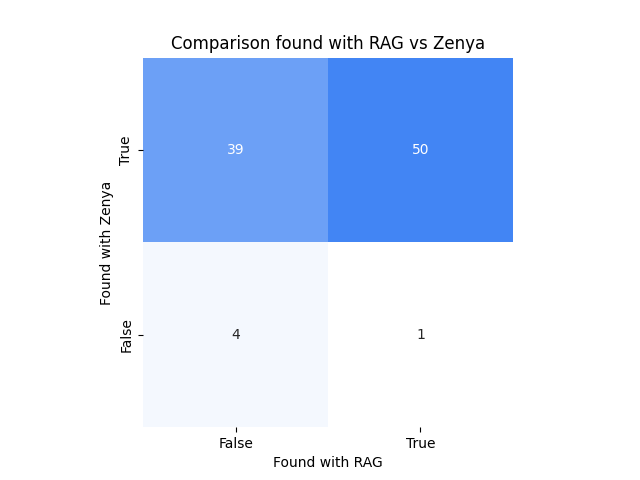
\includegraphics[width=0.9\linewidth]{fig/RAG_found_plot.png}}
    \caption{The distribution of all conversations, indicating whether the answer was found or not. This is illustrated for both the RAG system and the old system, Zenya.}
    \label{fig:found_rate}
\end{figure}

\begin{figure}[H]
    \centerline{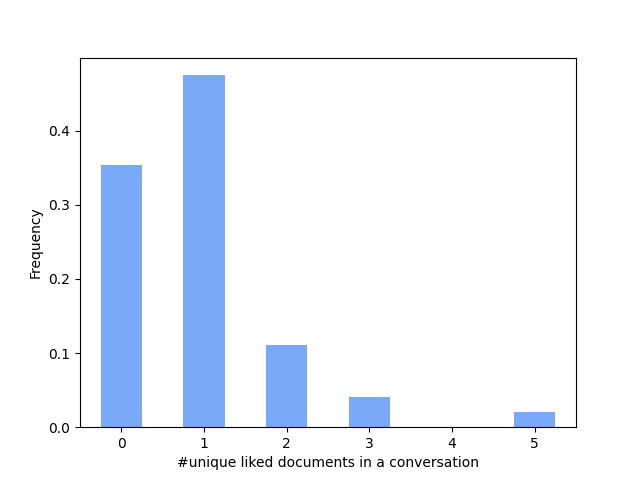
\includegraphics[width=0.7\linewidth]{fig/RAG_nr_correct_in_conversation.png}}
    \caption{Distribution of the number of unique correct documents found in a whole conversation. 0 means that no relevant document was found before the conversation was finished. If 1 or more correct documents were found (liked), it was a successful conversation.}
    \label{fig:liked_docs_per_convo}
\end{figure}

\begin{figure}[H]
    \centerline{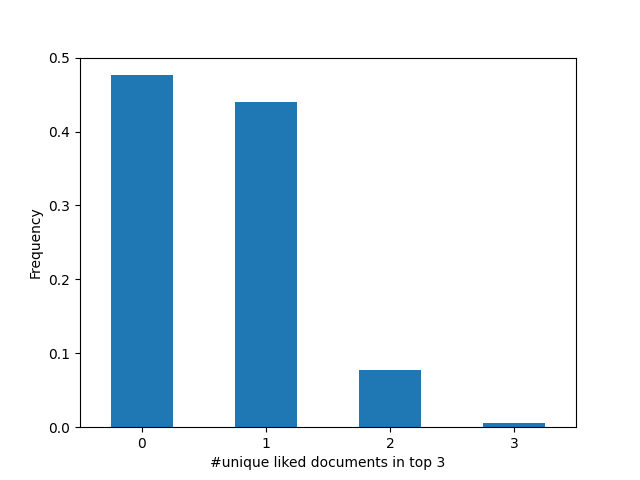
\includegraphics[width=0.7\linewidth]{fig/RAG_nr_top_3.png}}
    \caption{Distribution of the number of unique correct documents found per individual message. This is similar to the previous plot, but on the level of individual messages. If more than 1 document was correct (liked), it means that the question required parts from multiple documents to answer correctly and completely.}
    \label{fig:liked_docs}
\end{figure}

While the direct results are the most unfiltered, multiple red flags indicate that the statistics are not extremely reliable. For this reason, we filtered out the noise as follows, trying to remain completely unbiased in the process. All messages without any possible way of deducting the right document were left out, as approved by the UZGent. Combined with some manual labeling by the UZGent, the following results should be representative.

Figure \ref{fig:chunk_rank_density} and \ref{fig:chunk_rank_cumulative_distribution} show the same information with different emphasis: how the rank of the first relevant document is distributed. Figure \ref{fig:chunk_rank_density} shows the density. This visualization shows very well how most queries find the right document in the earlier ranks. When a document was not in the top 10, the chances clearly drop that the document is found at all. An important note to make is that a document not found is displayed as the maximal rank: 50, because by then we expect the doctor to never find it. With this information, one can see that about 10\% of the documents was totally not found. Figure \ref{fig:chunk_rank_cumulative_distribution} shows the cumulative distribution. This representation shows better what portion was already found by rank x. This shows the top 3 documents already have the right one 0.69\% of the time. We mention the Hit@3, because if the correct document is so highly ranked, it could be considered a perfect retrieval. The Hit@7 is 77\%, which again means 77\% of the times we have the right document in the top 7. We chose Hit@7, because after a Zenya query, the doctor sees 7 documents without scrolling any further. 90\% is found in the top 50 documents and as said before, 10\% are not found at all. The Hit@50 mostly shows how often a doctor could find a document at all, because they do not have time to scan beyond 50 titles.

\begin{figure}[H]
    \captionsetup{justification=centering}
    \centerline{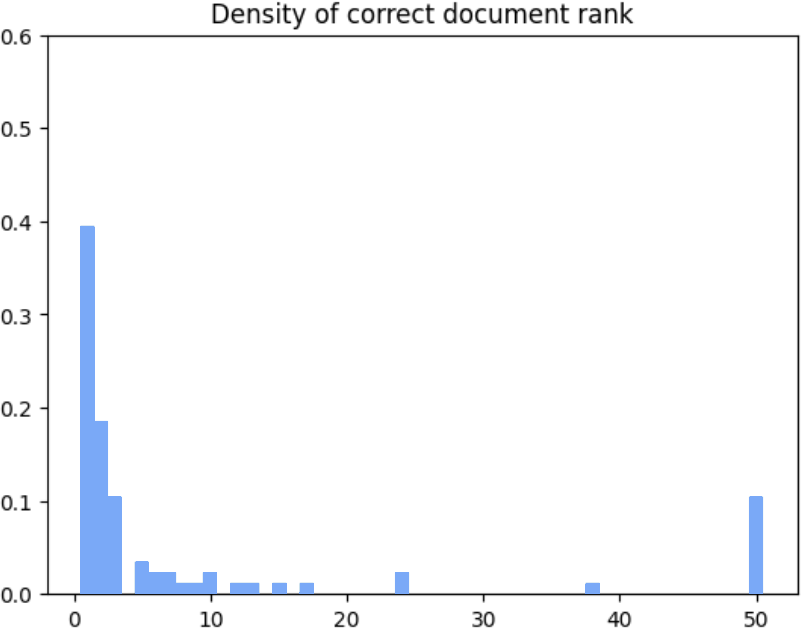
\includegraphics[width=0.7\linewidth]{fig/rag_distribution.png}}
    \caption{Distribution of the rank of the first correct document. More density to the left is better.}
    \label{fig:chunk_rank_density}
\end{figure}

\begin{figure}[H]
    \captionsetup{justification=centering}
    \centerline{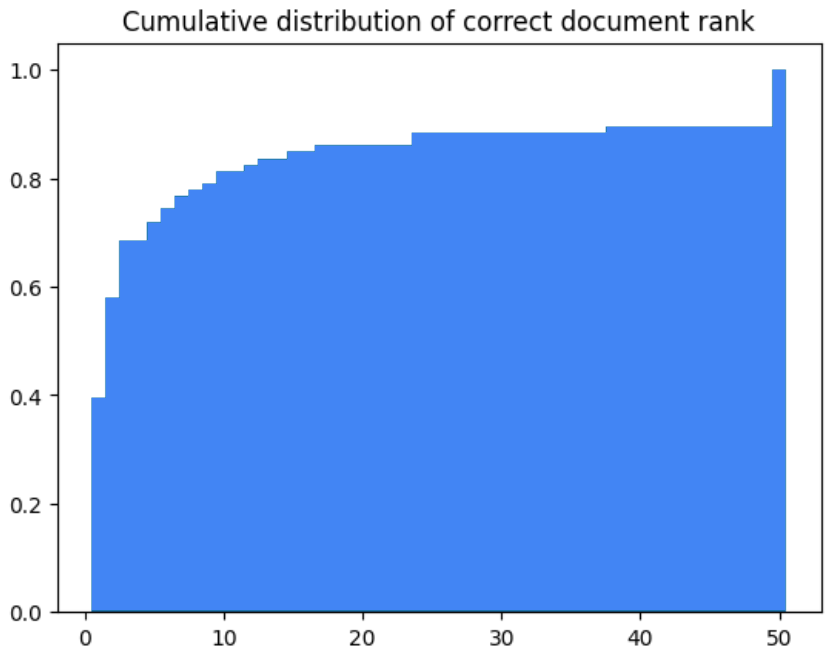
\includegraphics[width=0.7\linewidth]{fig/rag_cumulative_doc_rank.png}}
    \caption{Cumulative distribution of the rank of the first correct document, where the value shows the chance that a relevant document was somewhere in the top-k documents. Higher values are better.}
    \label{fig:chunk_rank_cumulative_distribution}
\end{figure}

The informal feedback provided great nuance to the objective feedback. The first and most important conclusion by most testers was that this system is not ready for production yet. As they were refering to the whole RAG system, this was a logical conclusion, given the large number of hallucinations. However, when asked about the retrieval only, the testers were more positive. Some were already convinced about the new model, while other still saw much work to be done. As a trend, the testers who work in a niche domain, were less convinced than the other ones. Interestingly, they said themselves that this problem could be very easily fixed by adding user information to the query. This means that a paediatrician should only get documents about children, or at least get them first. This information was not available, so it could not be implemented during the thesis. However, this is very important to be aware of for any future developer making retrievers for the UZGent.

One particular anecdote about the informal feedback really stood out: a nurse said that they are usually looking for five minutes in the current system, Zenya, before finding the right document, if it is found at all. While this was the most extreme example, the sentiment of the other testers seemed to be similar. They claimed that in the current system, one needs to know what they are looking for exactly, before searching or else one will never find the right document. This is of course the opposite of how a good retrieval system should work. The main conclusion out of this is that the results in Figure \ref{fig:found_rate} are to be taken with a grain of salt. For a fair comparison of both systems, one should choose testers who do not know either system yet. This will probably shift the results towards "not found" in Zenya, possibly even indicating our RAG system as the winner. Such tests are future work though.

Another type of feedback was implicit. Some testers asked how to pose their questions or just struggled finding a good question by themselves. This means asking a logical, natural language question is not as easy as first thought. Now, it must be said that the testers were biased. As they are Zenya experts that were trained for years to use only keywords, giving a natural language question to a computer just felt off for them.

\section{Future work at the UZGent and on the RAG system}
In this section, a list of ideas is given to the UZGent, should they be interested to further develop the RAG system.

The first step to do proper machine learning in general, is to have a high quality validate and test set. The sets we propose are a good start, but an increase in quantity is desirable. This is important, not only for further development, but also to compare other systems. For this reason, this is deemed to be the most important work, that needs to happen first. 

The next steps are ordered according to expected impact on the scores. As said before, adding metadata to the retriever's input could provide context that is necessary to retrieve the right document. Both metadata about the documents (which exists, but was not available during the thesis) and metadata about the user, which can be used to filter documents. Another extremely relevant improvement is to find a better embedder. While the currently used embedder is with reasonable certainty the best for the use case today, new great embedders pop up on HuggingFace every now and then. And as the difference between the best and second best embedder was immense, a new model might as well make such a large jump in the score.

As final recommendations for the UZGent we suggest the following. \textbf{Drop the generative model} and focus on improving the retriever. We see only advantages in this:
\begin{itemize}
    \item No risk of hallucinations. A retriever alone does not generate text and it leaves the responsibility to the doctors, who are more than capable to critically read the documents and asses the relevance.
    \item Reduced computational cost, both in terms of energy and latency.
    \item Reduced server requirements, which allows the application on a server with a cheap (or even no) GPU.
\end{itemize}
Even if generative language models were to be used in critical applications such as healthcare, we would advise to be very critical and only bring it to a production environment when it is objectively proven to be extremely accurate.

\section{Ethical considerations}
\label{Ethical considerations}
While the critical domain of healthcare brings many ethical considerations, this section will focus on one specifically: the hallucinations of the generator. For clear context: the demand for a RAG application came from the UZGent itself, before being implemented for this thesis. However, in the presented use case, we cannot afford critical mistakes with odds one to a million. As a typical generator hallucinates with much higher odds, a production-ready product was far out of scope of this thesis. For this reason, it is proposed only to work further with the retriever and to be very wary about any application that uses a generator directly to hand critical information to a healthcare professional. 

To make this suggestion more hands-on, some examples are given of good versus risky applications. A retriever using HyDE is good. There, the generator is used to augment the retriever and the final output is an existing document. As the documents are trustworthy, no wrong results are possible. Worst case, the wrong document is returned, the doctor sees this and then chooses another document. As a risky example, consider the RAG use case. Some documents are retrieved, then the generator makes an answer with them. The generator is the last step that gives possibly critical information. The generator could say anything wrong and if that were to be executed, it could have lethal effects. Now, one might say "make sure the answer is grounded in the context". That does not matter if it is looking at the wrong context. The best example is two documents, one for people of age up to 15 years old and another for people older than 15. These documents are semantically very close and contain nearly the same information making confusion very likely. Yet the doses could differ significantly and typical groundedness checks would not know it is looking at the wrong document. Another critical person could say ``but the healthcare professionals will notice, they have to check the sources for themselves''. First of all, people become lazy and stop checking the sources, that is just a fact. And even then, when it is required to find the answer in the document every time to verify, why is the answer even generated? All current ``solutions'' just seem like methods to boost confidence in the system, because mistakes are less likely (or at least seem less likely), yet more confidence just means more chance that when the system inevitably makes a mistake, it is trusted by the user.

While we do not advocate against any use of LLMs in these applications, we do urge to assess them with the necessary scrutiny. Only if objective measures are decisive, it can be brought to production.

